%% Tex spellcheck
% Maybe put this as Chapter 2

% Write in English.
\chapter{Chapter 1 :  Technical concepts}


\section{Magnetism}

Magnetism \footcite{noauthor_nasa_magnetism} is a physical phenomenon produced by the motion of electric charge, resulting in attractive and repulsive forces between objects. The motion of electric charge creates a magnetic field, which exerts a force on other moving charges.

The concepts of magnetism and electromagnetism are essential to the project. The board's design must take into account the magnetic fields generated by the coils and the magnets' attraction to these fields. For that we need to understand the basics of magnetism and electromagnetism. Ampere's Law for example states that the line integral of the magnetic field \(\mathbf{B}\) around a closed loop is proportional to the total electric current \(I\) passing through the loop. Mathematically, it is expressed as:

\[
	\oint_{\mathcal{C}} \mathbf{B} \cdot d\mathbf{l} = \mu_0 I_{\text{enc}}
\]

where:
\begin{itemize}
	\item \(\oint_{\mathcal{C}} \mathbf{B} \cdot d\mathbf{l}\) is the line integral of the magnetic field around a closed path \(\mathcal{C}\),
	\item \(\mu_0\) is the permeability of free space \((\mu_0 \approx 4\pi \times 10^{-7} \, \text{T} \cdot \text{m/A})\),
	\item \(I_{\text{enc}}\) is the total current enclosed by the path (in Amperes) \(\mathcal{C}\).
\end{itemize}

\newpage

\subsection{Direction of the magnetic field}
The direction of the current passing through a wire determines the direction of the magnetic field around the wire. The right-hand rule is a common way to determine the direction of the magnetic field around a current-carrying wire. The rule states that if the thumb of the right hand points in the direction of the current, the fingers will curl in the direction of the magnetic field around the wire.

\begin{figure}[H]
	\centering
	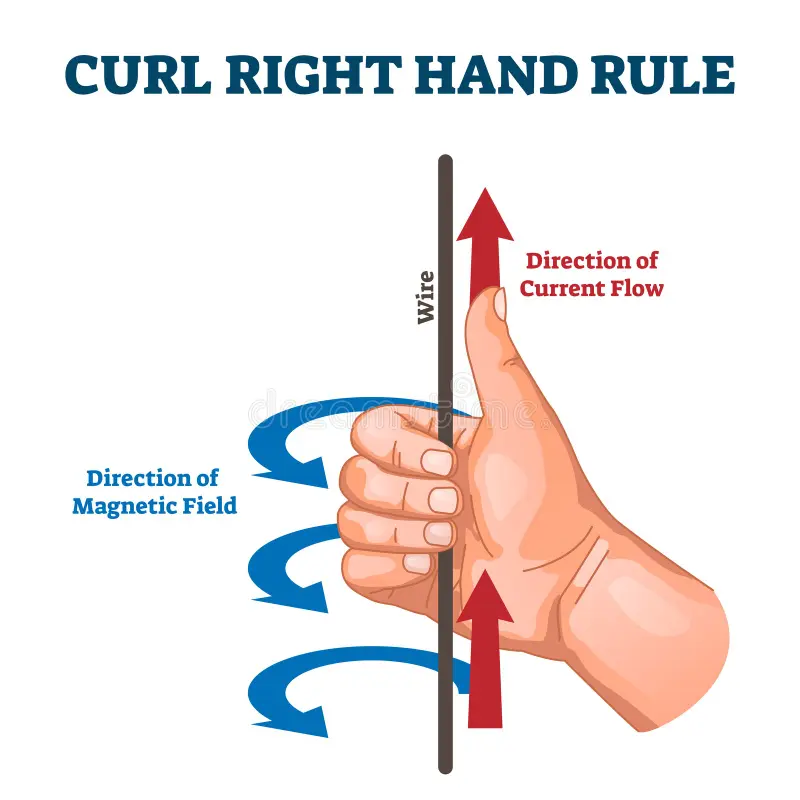
\includegraphics[width=0.6\linewidth]{right_hand.png}
	\caption[Right hand rule]{Right hand rule Source: thumbs.dreamstime.com ref: URL08}
	\label{fig:right_hand_rule}
\end{figure}


\section{Permanant magnets}

Permanent magnets are materials that produce a magnetic field without the need for an external magnetic field. They are made of ferromagnetic materials such as iron, nickel, and cobalt. The magnetic field is created by the alignment of the magnetic domains in the material. The domains align in the same direction, creating a net magnetic field. The strength of the magnetic field depends on the material and the alignment of the domains.

The strength of the magnetic field is measured in units of Tesla (T) or Gauss (G). Stacking magnets can increase the magnetic field strength\footcite{noauthor_factors_nodate}. For example, stacking flat disc magnets multiplies the adhesive force until the stack reaches a height of half the diameter of a single disc magnet at a maximum.

For testing purposes, we tried multiple magnets of different sizes from Super Magnet Shop\footcite{noauthor_buy_nodate}. The magnets come with a datasheet that give us the magnetic field strength of the magnets as Residual magnetism Br 13200-13700 G, 1.32-1.37 T. This means for example that the magnetic field strength of this specific magnet is between 1.32 and 1.37 Tesla.

They also give us the polarization pattern of the magnet. For example the disk magnet has its poles on the flat faces of the disk.

\begin{figure}[H]
	\centering
	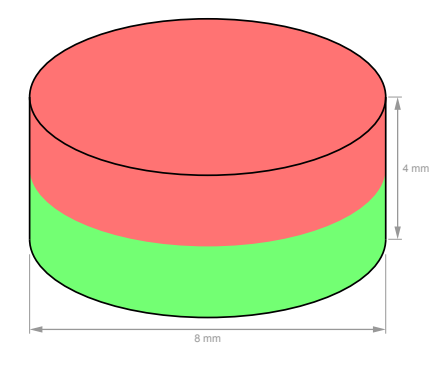
\includegraphics[width=0.6\linewidth]{disk.png}
	\caption[Disk magnet polarity]{Disk magnet polarity Source: www.supermagnete.ch ref: URL09}
	\label{fig:disk}
\end{figure}

\begin{figure}[H]
	\centering
	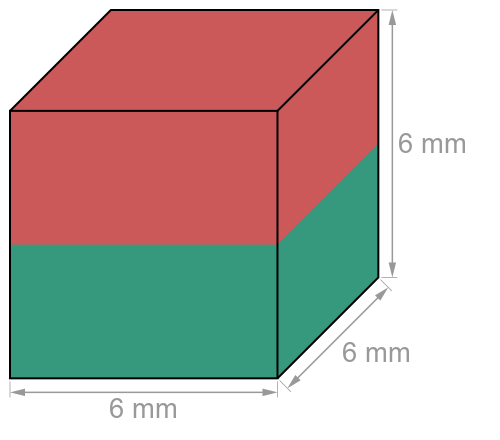
\includegraphics[width=0.6\linewidth]{cube.png}
	\caption[Cube magnet polarity]{Cube magnet polarity Source: www.supermagnete.ch ref: URL09}
	\label{fig:cube}
\end{figure}

\section{Calculate the force of a magnetic field on a magnet}

To calculate the force exerted on a magnet by a magnetic field (for example from a pcb coil), taking into account friction and the magnet's mass, we can use the following formulas:

Calculate the Magnetic Force

\[
	F_{\text{mag}} = m \cdot B \cdot \sin(\theta)
\]

Calculate the Friction Force

\[
	F_{\text{friction}} = \mu \cdot m_{\text{weight}} \cdot g
\]

Calculate the Total Force

\[
	F_{\text{total}} = F_{\text{mag}} - F_{\text{friction}}
\]

